\subsection{Pilot Aleatoric UQ Usecase}
\label{sec:pilot_uq_usecase}

Two deliverables, one study:

\begin{enumerate}
  \item \textbf{Exercise GridKit as an end user} \cite{GridKit2025} on a problem it has not been pointed at before, and report back what works and what does not.
  \item \textbf{Demonstrate aleatoric UQ by sampling} \cite{DerKiureghian2009} on a dynamics problem, and find out where the sampling cost actually goes --- with a view to much larger grids where brute force stops being an option.
\end{enumerate}

The vehicle is a question utilities are being asked right now \cite{Shehabi2024}:

\begin{quote}
\textbf{Where, and how much, large datacenter load can be added before dynamic security degrades --- given that renewable output makes system inertia vary hour to hour?} \cite{Milano2018}
\end{quote}

This is a pilot. The grid is small, the contingency set is narrow, and several conclusions are bounded by model validity. The point is to establish the machinery and learn where the difficulty lives.

\subsection{Glossary}
\label{sec:glossary}

Main terms used in our pilot study that follows.

\begin{description}
  \item[\textbf{Operating condition}] One (hour, commitment) pair. The hour fixes load and wind; the commitment fixes which thermal units are online.
  \item[\textbf{Placement}] Where the datacenter sits: none (the baseline), bus 108 or bus 148 in the fault sweep, or one of buses 6, 108, 120 and 148 in the aleatoric campaign. Not a property of the operating condition.
  \item[\textbf{Scenario}] One operating condition with one placement, e.g. hour 204, commitment 27, datacenter at bus 108. It is the unit the pilot's five rows describe. Each scenario is run against all faults.
  \item[\textbf{Baseline}] The \textit{no-datacenter} run \textbf{for a given operating condition} --- not one global reference. Each condition has its own, so \texttt{dCCT} compares like with like.
  \item[\textbf{Net load}] Demand minus wind, system-wide. What the thermal fleet must serve.
  \item[\textbf{CCT}] Critical clearing time: the longest fault the system survives. Larger is safer.
  \item[\textbf{Fault duration}] How long the fault stays on before it is cleared, in seconds. Stored as \texttt{fault\_\allowbreak{}duration\_\allowbreak{}s}. The pilot campaigns run each row at 0.1 s. The CCT search sets its own durations in \texttt{[0.05, 0.5]} s ({\textsection}5).
  \item[\textbf{h-scale}] Multiplier on every generator's inertia constant \texttt{H} in the case. \texttt{1.0} is the base case, stored as \texttt{h\_\allowbreak{}scale}. All pilot rows use \texttt{1.0}.
  \item[\textbf{Nadir}] The lowest system frequency reached after the fault, taken as the mean bus frequency (a proxy for the centre-of-inertia frequency), after the post-fault blank window. Higher is safer. Recorded, but not the stability test ({\textsection}11).
  \item[\textbf{ROCOF}] Rate of change of frequency, \texttt{|d f / dt|} of that mean bus frequency in Hz/s, maximum after the blank window. Fast change means little inertia to absorb the imbalance. Recorded, but not the stability test ({\textsection}11).
  \item[\textbf{The cap}] \texttt{cct\_\allowbreak{}max = 0.5 s}, the top of the search. Set at a credible protection time; we do not look past it.
  \item[\textbf{Censored}] \textbf{CCT is at or above the cap} --- the system survived the longest fault we consider. The stored \texttt{0.5} is a \textbf{lower bound, not a measurement}. Censored means \textit{very stable}.
  \item[\textbf{Uncensored pair}] A (baseline, sited) pair where \textbf{both} are measured, so \texttt{dCCT} is a number rather than an inequality.
  \item[\textbf{Hosting capacity}] Largest datacenter MW at a bus that is both deliverable and secure.
  \item[\textbf{\texttt{LOCALLY\_\allowbreak{}INFEASIBLE}}] The OPF cannot serve the load at all. A \textbf{result} (deliverability binds), not an error.
  \item[\textbf{Stage A / B / C}] The stage a parameter binds at: \textbf{A} = the dispatch (dispatch, which needs a Julia solve), \textbf{B} = the \texttt{case.json} edit, \textbf{C} = the dynamic re-run.
  \item[\textbf{ZIP}] Load model shares \texttt{alphaZ}/\texttt{alphaI}/\texttt{alphaP} (constant impedance / current / power), summing to 1. Written \texttt{P/I/Z}. The pilot's datacenter mix is \texttt{80/20/0} ({\textsection}4.4).
  \item[\textbf{Main campaigns}] \texttt{aleatoric1\_\allowbreak{}ap08\_\allowbreak{}qlim} and \texttt{faultscreen1\_\allowbreak{}ap08\_\allowbreak{}qlim}: DC OPF, then AC PF with PV$\to$PQ switching, datacenter at \texttt{P/I/Z = 80/20/0}, alphaP 0.8. The headline numbers are read against these ({\textsection}7.0).
  \item[\textbf{DC OPF / AC PF}] DC OPF sets \textit{who generates} from active power only (lossless, no voltages, no Q). AC PF takes that dispatch and solves the voltages and reactive power.
  \item[\textbf{PV bus / PQ bus}] PV: the generator fixes P and voltage magnitude, and Q is whatever holds the voltage. PQ: P and Q are fixed (a load); voltage is a result.
  \item[\textbf{Q limit}] A generator's maximum (\texttt{QMAX}, field-current heating) and minimum (\texttt{QMIN}, stator end-region heating) reactive output.
  \item[\textbf{PV$\to$PQ switching}] When a generator's Q leaves its limits, it is fixed at the limit and its bus is solved as PQ. Standard in planning tools; the pipeline's version is in {\textsection}4.2.
\end{description}

\vspace{-0.3em}
\noindent\fbox{\parbox[t]{0.98\textwidth}{%
\setlength{\parskip}{0pt}%
\textbf{Details:} \url{https://github.com/ORNL/GridKit/blob/isatkaus/uq-usecase/uq-usecase/work-notes/datacenter_load_uq_plan.md}. Sections: "physical intuition"
}}
\vspace{-0.2em}
\subsection{The system}
\label{sec:the_system}

ACTIVSg200, a synthetic Illinois case \cite{Birchfield2017}: \textbf{200 buses, 246 branches, 49 generators} (25 coal, 17 natural gas, 6 wind, 1 nuclear). The seed dispatch totals \textbf{2,178 MW} of demand, which is the annual peak. The dynamic case (\texttt{ACTIVSg200.case.json}) carries \textbf{40 Genrou} machines: 34 thermal and the 6 wind units, which the campaign replaces with negative LoadZIP stand-ins ({\textsection}4.3), leaving \textbf{34 synchronous machines}. The 9 thermal units offline in the seed \texttt{.m} (\texttt{GEN\_\allowbreak{}STATUS = 0}) have no machine in the case and were not added in these experiments. The JSON also carries \textbf{109 LoadZIP} loads, before the wind stand-ins are added.

Hourly load and wind come from an 8,760-hour dataset for this footprint, so the (demand, wind) joint distribution is empirical rather than assumed.

\subsubsection{One-time seed building}

The shipped case is not used directly. Once per case, it is rebuilt from the two TAMU source files, and the rebuild is checked against the shipped \texttt{case.json}. That gives two artifacts. The \textbf{base case} supplies every machine's dynamic parameters. The \textbf{seed \texttt{.m}} supplies the dispatch: which units are online and how much they produce. Each condition then overwrites only the dispatch, on a copy of the base case. Blue boxes are the one-time build; grey boxes run per condition.

\begin{figure}[htb]
  \centering
  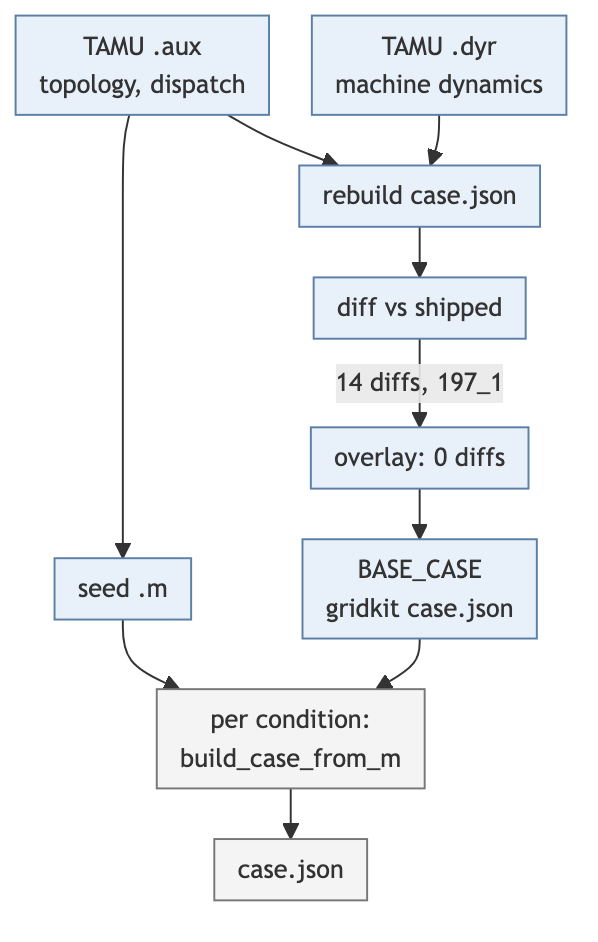
\includegraphics[width=0.60\textwidth]{figs/fig:3_one_time_seed_building_blue_and_the_pe.png}
  \par\vspace{0.4em}
  {\small Figure 3.1. One-time seed building (blue) and the per-condition build (grey).}
\end{figure}

What we change relative to what ships:

\begin{itemize}
  \item \textbf{Dynamics come from the base case, not the shipped file.} The rebuild differs from the shipped file in 14 parameters, all on machine \texttt{197\_\allowbreak{}1}. The author's values are kept by overlay, so the base case equals the shipped file.
  \item \textbf{The dispatch is overwritten per condition.} The \texttt{.m} cannot store machine inertia, so dynamics are always inherited from the base case.
  \item \textbf{Six wind units become negative load stand-ins} ({\textsection}4.3), so they carry no inertia.
\end{itemize}

\par\vspace{0.8em}
\noindent\fbox{\parbox[t]{0.95\textwidth}{%
\setlength{\parskip}{0.3em}%
\setlength{\baselineskip}{1.15\baselineskip}%
\textbf{Details:} \url{https://github.com/ORNL/GridKit/blob/isatkaus/uq-usecase/uq-usecase/work-notes/datacenter_load_uq_plan.md}. Sections: "where the wind timeseries came from", "the operating-condition space", "why 8760 is not a sampling design"
}}
\vspace{0.3em}

\par\vspace{0.8em}
\noindent\fbox{\parbox[t]{0.95\textwidth}{%
\setlength{\parskip}{0.3em}%
\setlength{\baselineskip}{1.15\baselineskip}%
\textbf{Details:} \url{https://github.com/ORNL/GridKit/blob/isatkaus/uq-usecase/uq-usecase/work-notes/m_to_case_helper.md}. Sections: "where validation checks are"
}}
\vspace{0.3em}
\subsection{Building one operating condition}
\label{sec:building_condition}

\begin{figure}[htb]
  \centering
  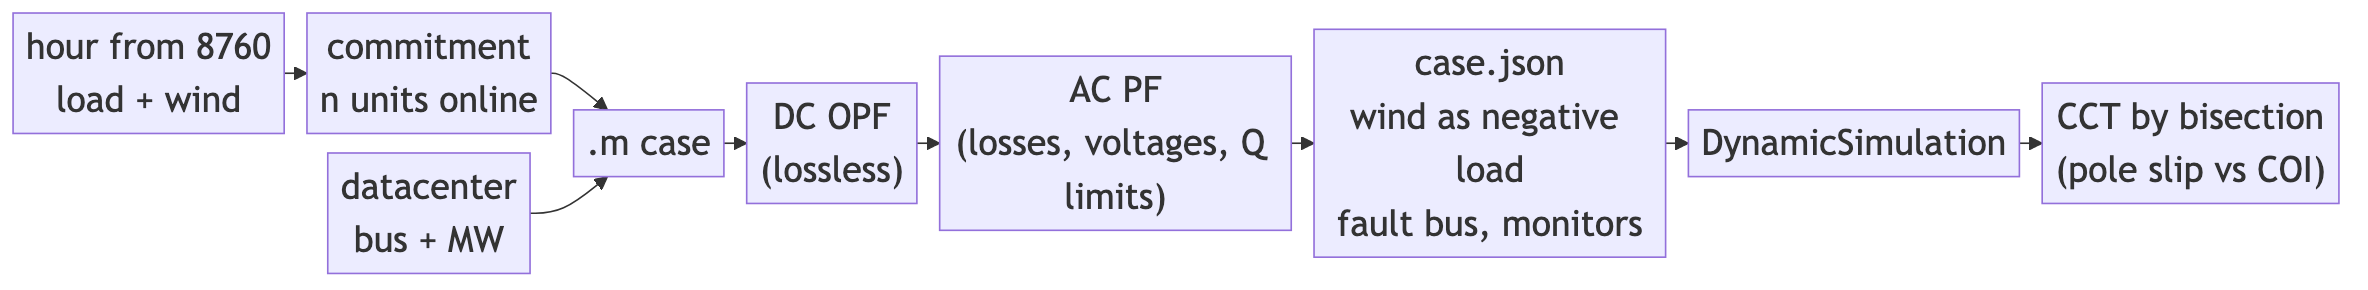
\includegraphics[width=0.95\textwidth]{figs/fig:4_per_condition_pipeline_from_hour_and_co.png}
  \par\vspace{0.4em}
  {\small Figure 4.1. Per-condition pipeline, from hour and commitment to CCT. Nadir, ROCOF and Vmin are also recorded but do not set CCT.}
\end{figure}

\subsubsection{Commitment: a feasible band, not an economic optimum}
\label{sec:commitment}

We do \textbf{not} solve a unit-commitment MILP. We compute the band of \textit{feasible} commitments and sample across it:

\begin{itemize}
  \item \textbf{lower bound} --- adequacy (\texttt{capacity >= net x 1.10}) and a floor of 8 thermal units, below which the network loses voltage support and the integrator fails to initialise \cite{Hindmarsh2005};
  \item \textbf{upper bound} --- \texttt{sum(PMIN) <= net}, above which the OPF is infeasible.
\end{itemize}

At 762 MW net load the band is \texttt{[18, 38]}. Both ends are legitimate: at \texttt{n = 33} the committed minimums total 740 MW, still under the load, so the units simply run further down their range.

\textbf{How commitment is sampled.} For each sampled hour, the band is computed from that hour's own net load (demand minus wind). The campaign then commits at two fixed positions in the band, 0.25 and 0.75 of the way from \texttt{n\_\allowbreak{}min} to \texttt{n\_\allowbreak{}max}, rounded to whole units. So each hour gives two operating conditions. This is a stratified choice at fixed positions, not a uniform draw from the band and not a draw from an assumed distribution. The fault sweep (\texttt{faultscreen1\_\allowbreak{}ap08\_\allowbreak{}qlim}, {\textsection}7.5) uses 10 hours $\times$ 2 commitments = 20 conditions. Its realised positions are 0.22 to 0.28 of the band, after rounding to whole units. The aleatoric campaign (\texttt{aleatoric1\_\allowbreak{}ap08\_\allowbreak{}qlim}, {\textsection}7.0) uses 20 hours $\times$ 2 commitments = 40 conditions. Hours are stratified by net-load quintile with equal counts per quintile (2 each in the fault sweep, 4 each in the aleatoric campaign), so each quintile carries equal weight, matching the empirical net-load distribution. The aleatoric campaign's hours were drawn at random (seed 0). In both campaigns the datacenter arms reuse the baseline commitment of their hour.

\textbf{Why commitment matters.} A commitment sets which thermal units are online, and so the inertia and headroom on the system. A low-load hour can run many units at part load, carrying more inertia, or run few, carrying less. Both are feasible, and a single committed point would hide that spread. At hour 4779 (762 MW net load), the two ends of the band are:

\vspace{0.15cm}
\centering\small
\setlength{\tabcolsep}{8pt}
\begin{tabular}{lll}
commitment & fleet inertia & mean output per unit \\
\midrule
n = 23 & \textbf{7,512 MW$\cdot$s} & 33.1 MW \\
n = 33 & \textbf{11,702 MW$\cdot$s} & 23.1 MW \\
\end{tabular}
\vspace{0.15cm}
\normalsize\raggedright

They differ by a \textbf{factor of 1.56 in inertia at identical load and wind}. The n = 33 value is the pre-correction formula value, which the plan measured 1.4 \% low at hour 6164, so the true ratio is likely slightly higher. That is the dominant lever on stability at fixed net load. We have real data for the net-load distribution but none for how this synthetic system's operators would commit, so inventing a commitment PDF would fabricate the very thing that drives the answer. Results are reported \textbf{conditionally} on commitment and can be reweighted later if a real UC distribution appears.

Adding a datacenter does \textbf{not} change the commitment. The same \texttt{n} units stay online, and only the dispatch is re-solved (DC OPF, then AC PF). If the committed fleet cannot serve the added load, the case is recorded as infeasible, not re-committed. Those failures therefore overstate what an operator could do by committing more units.
\par\vspace{0.8em}
\noindent\fbox{\parbox[t]{0.98\textwidth}{%
\setlength{\parskip}{0pt}%
\textbf{Details:} \url{https://github.com/ORNL/GridKit/blob/isatkaus/uq-usecase/uq-usecase/work-notes/datacenter_load_uq_plan.md}. Sections: "how commitment is sampled", "why the band is so wide, and why we sample inside it", "commitment is a first-order driver (Phase 1b inertia sweep)"
}}
\vspace{0.2em}
\subsubsection*{0.0.4.2 Dispatch: DC OPF then AC PF}
\addcontentsline{toc}{subsubsection}{0.0.4.2 Dispatch: DC OPF then AC PF}
\label{sec:dispatch_dc_opf_ac_pf}

\noindent\fbox{\parbox[t]{0.98\textwidth}{%
\setlength{\parskip}{0pt}%
\textbf{Implementation note:} Currently, the dispatch pipeline uses PowerModels.jl for both DC OPF and AC PF solves. As OPF functionality becomes available in GridKit (currently under development), we can readily substitute it into the pipeline. Maintaining PowerModels.jl as an alternative is beneficial for validation purposes and exploration of various AC OPF relaxation formulations.
}}
\vspace{0.4em}

Both solves use PowerModels.jl \cite{Coffrin2018} with Ipopt \cite{Wachter2006}. Per condition:

\begin{enumerate}
  \item \textbf{DC OPF} sets the economic dispatch. It is lossless, so the load is inflated by the loss estimate from the previous pass (zero on the first).
  \item \textbf{AC PF} solves the real network at that dispatch, giving voltages, Q and the actual losses. The losses feed the next DC OPF.
\end{enumerate}

\textit{Figure 4.2} shows the loop. With \texttt{loss\_\allowbreak{}iters = 1} there is one correction, so each condition runs two DC OPFs and two AC PFs.

\begin{figure}[htb]
  \centering
  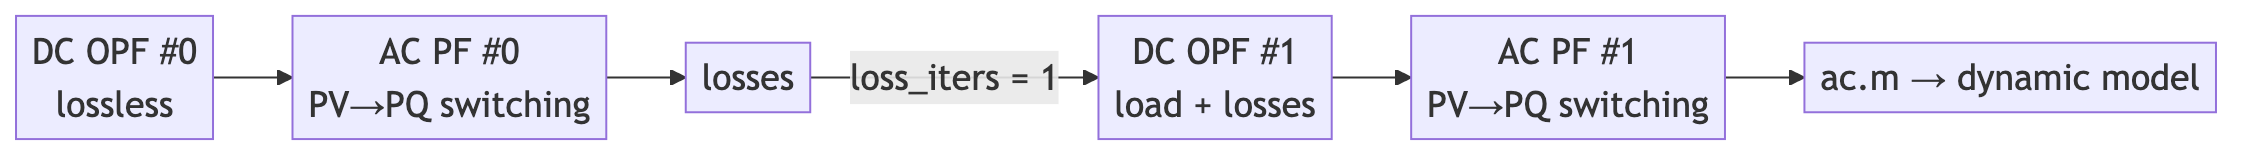
\includegraphics[width=0.95\textwidth]{figs/fig:4_dispatch_loop_per_condition_dc_opf_ac.png}
  \par\vspace{0.4em}
  {\small Figure 4.2. Dispatch loop per condition: DC OPF, AC PF, one loss correction, AC PF. Each AC PF restarts its PV$\to$PQ switching from all units at PV.}
\end{figure}

The iteration exists because of a \textbf{slack problem}: a power flow leaves one generator's P free, so it structurally cannot enforce \texttt{PMAX} on the slack, and our slack is the nuclear unit \texttt{189\_\allowbreak{}1} with \textbf{0.0082 MW} of headroom. Without re-dispatch it would absorb the entire loss term, and in an hourly loop the whole load change. One loss correction reduces the overshoot from 27.05 MW to 0.34 MW on the worst hour (0.016 \% of load), which is why \texttt{loss\_\allowbreak{}iters = 1}. A second correction reduces it only to 0.005 MW.

\textbf{Why we use switching, not AC OPF.} We tested AC OPF as an alternative Q-limit route (discussed further below). AC OPF changes dispatch (about 280 MW summed in the pilot), so a CCT difference cannot be attributed to Q limits alone. Switching keeps the DC OPF dispatch and changes only Q, isolating the Q-limit effect that this report asks about. AC OPF stays in the pipeline as the \texttt{ac\_\allowbreak{}opf} option for cross-checks.

\textbf{Reactive limits: PV$\to$PQ switching.} AC power flow does not enforce generator \texttt{QMAX}/\texttt{QMIN} limits natively (measured: 2 to 11 violations per scenario without mitigation). We enforce them via PV$\to$PQ switching \cite{Stott1974}: after solving voltages, any generator exceeding a Q limit is fixed at that limit and its bus switched to PQ, then re-solved. Fixed generators return to PV if voltage recovers past setpoint (repeat up to twice). The DC OPF dispatch is never changed---only Q adjusts. This preserves dispatch so that CCT differences from the unlimited-Q run can be attributed to reactive limits alone. The feature is on by default (\texttt{enforce\_\allowbreak{}q\_\allowbreak{}lims}) in the main campaigns but disabled in unlimited-Q studies.

\textbf{AC OPF as a second Q-limit route.} PowerModels.jl's AC OPF enforces Q limits as constraints, replacing DC OPF + AC PF + switching. We built it as an opt-in path (\texttt{ac\_\allowbreak{}opf}) but did not adopt it for the main campaigns: AC OPF changes dispatch ($\sim$280 MW summed in the pilot), making it impossible to isolate Q-limit effects from dispatch effects. Switching preserves dispatch and changes only Q ($\sim$0.82 MW loss variation), cleanly answering the report's question. AC OPF remains as a cross-check and can be reported if needed.
\par\vspace{0.8em}
\noindent\fbox{\parbox[t]{0.98\textwidth}{%
\setlength{\parskip}{0pt}%
\textbf{Details:} \url{https://github.com/ORNL/GridKit/blob/isatkaus/uq-usecase/uq-usecase/work-notes/datacenter_load_uq_plan.md}. Sections: "the dispatch chain", "the slack problem", "the loss-iteration fix, with convergence table", "why DC OPF then AC PF, rather than AC OPF"
\textbf{Details:} \url{https://github.com/ORNL/GridKit/blob/isatkaus/uq-usecase/uq-usecase/work-notes/datacenter_load_uq_plan.md}. Sections: "switching implementation and five-scenario measurements", "pipeline code", "Q-limit fold recount"
\textbf{Details:} \url{https://github.com/ORNL/GridKit/blob/isatkaus/uq-usecase/uq-usecase/work-notes/datacenter_load_uq_plan.md}. Sections: "AC OPF design and pilot results"
}}
\vspace{0.2em}
\subsubsection*{0.0.4.3 Wind becomes negative load}
\addcontentsline{toc}{subsubsection}{0.0.4.3 Wind becomes negative load}
\label{sec:wind_negative_load}

\noindent\fbox{\parbox[t]{0.98\textwidth}{%
\setlength{\parskip}{0pt}%
\textbf{Implementation note:} The ACTIVSg200 case lacks native renewable energy converter controls models for wind and photovoltaic units. GridKit implements comprehensive IBR models---specifically REGCA (converter control), REECB (reactive power and volt/var support), and REPCA (plant control)---which have been implemented and unit-tested in the codebase. Substituting these proper RECC models for the current constant-current stand-in is straightforward and will be readily incorporated in future campaigns to improve fidelity of inverter-based resource dynamics.
}}
\vspace{0.4em}

Wind units are removed as \texttt{Genrou} machines and re-inserted as a \textbf{negative \texttt{LoadZIP}} at their own bus, with \texttt{alphaI = 1} (constant current). Left as synchronous machines, they could contribute \textbf{up to 2,766 MW$\cdot$s} of inertia at their ratings (sum over the 6 wind Genrou units of \texttt{H} $\times$ \texttt{mva}), whatever the wind output, and inertia is what the study varies. Constant power made the integrator fail at high wind penetration.

\textbf{Implementation.} Hourly wind MW is pinned in the DC OPF, the AC power flow solves its reactive output, and the solved P and Q are written into the ZIP. Stage B rewrites \texttt{case.json}: each wind unit's \texttt{Genrou}, \texttt{Tgov1} and \texttt{SexsPti} are removed and a \texttt{LoadZIP} is added with \texttt{Pnom = -PG/100} and \texttt{Qnom = -QG/100} (per unit, 100 MVA base), \texttt{alphaI = 1}, \texttt{alphaP = 0}. GridKit treats positive \texttt{Pnom} as consumed, so the negative value injects PG. At the initial voltage this reproduces the power-flow P and Q exactly; after that the injection scales with \texttt{|V|}, which is constant current.

\textbf{Why it is acceptable.} Converter-interfaced generation is modelled in positive-sequence transient stability as a controllable current source \cite{Pourbeik2017}. The Sandia PSTess manual says that, \textit{"as in the WECC REGC\_A model"}, the converter interface is "a controllable current source" \cite{Elliott2021}. A constant-current ZIP is a simple stand-in for that current injection.
\par\vspace{0.8em}
\noindent\fbox{\parbox[t]{0.98\textwidth}{%
\setlength{\parskip}{0pt}%
\textbf{Details:} \url{https://github.com/ORNL/GridKit/blob/isatkaus/uq-usecase/uq-usecase/work-notes/datacenter_load_uq_plan.md}. Sections: "wind pipeline, function by function", "wind: why negative load, not fixed", "implementation", ""net load" is an aggregate, not a per-bus subtraction"
}}
\vspace{0.2em}
\subsubsection*{0.0.4.4 The datacenter}
\addcontentsline{toc}{subsubsection}{0.0.4.4 The datacenter}
\label{sec:datacenter}

\noindent\fbox{\parbox[t]{0.98\textwidth}{%
\setlength{\parskip}{0pt}%
\textbf{Implementation note:} The GridKit team has plans to develop comprehensive dynamic models for datacenter loads. Once implemented and validated, these models will be readily incorporated to replace the quasi-static ZIP approximation and improve system response fidelity.
}}
\vspace{0.4em}

A datacenter is represented as \textbf{additional electrical load placed at one bus}. Two things about \textit{how} it is added matter to the answer.

\textbf{It is added before dispatch, not after.} The load enters the network data that the optimiser sees, so the commitment and the dispatch must produce and deliver the extra power. If it were added after dispatch, neither the commitment nor the OPF would see it: the power flow would have the slack bus supply it, and the committed fleet could be too small to serve it or larger than needed.

\textbf{It gets its own load device, with its own voltage behaviour.} Load in these cases is represented by a \textbf{ZIP model} \cite{IEEELoad1993}, which splits demand into three parts by how each responds when voltage sags: a constant-\textbf{impedance} part (falls as $V^2$), a constant-\textbf{current} part (falls as $V$), and a constant-\textbf{power} part (does not fall at all). The split is written here as \texttt{P/I/Z} percentages.

The distinction is the physical reason a datacenter is interesting. Ordinary constant-impedance load \textit{sheds itself} during a voltage dip and helps the system recover. Datacenter load is rectifier- and UPS-fed and behaves far closer to constant power \cite{Milanovic2013}: it keeps demanding the same megawatts at reduced voltage, which means drawing more current, which depresses voltage further. If the new load were simply folded into whatever device already existed at the bus, it would inherit the host's helpful constant-impedance behaviour and the study would measure the wrong thing. So the datacenter gets a \textbf{separate} device, and the host device is left as it was.

\textbf{Every load device in the shipped case is constant impedance.} All 109 \texttt{LoadZIP} devices in \texttt{ACTIVSg200.case.json} have \texttt{alphaI = alphaP = 0}, so \texttt{alphaZ = 1}. Before any datacenter is added, every host load is pure constant impedance.

\textbf{How the datacenter reaches the model.} The MW is added to the bus's demand in the \texttt{.m} before dispatch, so the OPF has to serve it. The network build then folds all demand at each bus into one \texttt{LoadZIP}, host plus datacenter together. \texttt{split\_\allowbreak{}out\_\allowbreak{}datacenter} subtracts the datacenter's MW and MVAr from that device, which restores the original host load, and appends a second device for the datacenter. The end state is the original host (N1, \texttt{alphaZ = 1}) beside the datacenter (N2, \texttt{P/I/Z = 80/20/0}). That is the same as adding an N2 device beside an untouched N1; the subtraction only undoes the fold. A bus with no load has no host to restore, and the datacenter device is the only one.

\par\vspace{0.4em}
\noindent\fbox{\parbox[t]{0.98\textwidth}{%
\setlength{\parskip}{0pt}%
\textbf{Details:} \url{https://github.com/ORNL/GridKit/blob/isatkaus/uq-usecase/uq-usecase/work-notes/datacenter_load_uq_plan.md}. Sections: "datacenter pipeline, function by function", "placement selection"
}}
\vspace{0.2em}

\textbf{Placement.} The candidate pool is the 16 load-carrying buses of the \texttt{phase3b} siting sample. The two main campaigns use subsets of it:

\begin{itemize}
  \item the fault sweep (\texttt{faultscreen1\_\allowbreak{}ap08\_\allowbreak{}qlim}, {\textsection}7.5): buses 108 and 148, at 200 MW;
  \item the aleatoric campaign (\texttt{aleatoric1\_\allowbreak{}ap08\_\allowbreak{}qlim}, {\textsection}7.0): buses 6, 108, 120 and 148, at 50, 100, 200, 300 or 400 MW.
\end{itemize}

\textbf{The pilot mix is \texttt{P/I/Z = 80/20/0}.} The physically intended model is pure constant power, \texttt{100/0/0}. It is not simulable at every bus (see section 8), and folds grow with \texttt{alphaP} (hunt summary below), so \texttt{alphaP} 1.0 fails more initial-condition solves. The campaigns therefore use 80\% constant power and 20\% constant current, with no constant impedance. The 20\% constant-current share rests on a plausible but unverified argument: a converter-fed load reaches its current limit in a deep dip, and a current-limited converter behaves as constant current. The 20\% is a choice, not a fitted value. The earlier campaigns used \texttt{20/80/0}, now a sensitivity case; its effect on CCT is in the plan.

\textbf{Hunt summary (IDA initial-condition failures at high \texttt{alphaP}).} At high \texttt{alphaP}, the datacenter shifts the network-algebraic fold past a bolted fault, creating no-steady-state outcomes that limit where datacenters can be sited.

\par\vspace{0.4em}
\noindent\fbox{\parbox[t]{0.98\textwidth}{%
\setlength{\parskip}{0pt}%
\textbf{Details:} \url{https://github.com/ORNL/GridKit/blob/isatkaus/uq-usecase/uq-usecase/work-notes/datacenter_load_uq_plan.md}. Sections: "fold hunt summary: IDA initial-condition failures at high alphaP", "IDA initial-condition issue record", "results", "hypothesis"
}}
\vspace{0.2em}

\par\vspace{0.4em}
\noindent\fbox{\parbox[t]{0.98\textwidth}{%
\setlength{\parskip}{0pt}%
\textbf{Details:} \url{https://github.com/ORNL/GridKit/blob/isatkaus/uq-usecase/uq-usecase/work-notes/datacenter_load_uq_plan.md}. Sections: "ZIP coefficients are a first-class lever", "is the 20/80/0 mix defensible?", "Phase 3: datacenter dimension", "what is sampled, and what is chosen", "design of the sweep", "two limits, and the thermal one binds first"
}}
\vspace{0.2em}

\subsection{CCT by bisection}
\label{sec:cct_bisection}

Critical clearing time is found by bisecting fault duration in \texttt{[0.05, 0.5]} s, with a stability test of \textbf{pole slip relative to the centre of inertia} \cite{Kundur2004}, \cite{Kundur1994}. The centre of inertia \cite{SauerPai1998} is the inertia-weighted average rotor angle of the fleet,


\[
\delta_{COI}(t) = \frac{\sum_i H_i S_i \delta_i(t)}{\sum_i H_i S_i}
\]

and a run is declared unstable when any machine leaves that collective frame:


\[
\max_{i,\,t} \bigl| \delta_i(t) - \delta_{COI}(t) \bigr| > 180^{\circ}
\]

Every symbol maps to a GridKit name or to a derived quantity:


\vspace{0.25cm}
\centering\small
\renewcommand{\arraystretch}{1.25}
\begin{tabularx}{\textwidth}{l >{\raggedright\arraybackslash}X >{\raggedright\arraybackslash}X}
\toprule
    Symbol & Meaning & GridKit name, and where it is read \\
\midrule
    $i$ & one of the 26 Genrou machines in ACTIVSg200 & \texttt{Genrou} device \texttt{id}, e.g. \texttt{49\_\allowbreak{}1\_\allowbreak{}genrou} \\
    $H_i$ & inertia constant, in s & \texttt{H} in \texttt{params} of device $i$ in \texttt{case.json} \\
    $S_i$ & machine MVA base & \texttt{mva} in \texttt{params} of device $i$ in \texttt{case.json} \\
    $\delta_i(t)$ & rotor angle of machine $i$ & Genrou state \texttt{delta} (radians), monitor column \texttt{Genrou\_\allowbreak{}<device id>\_\allowbreak{}delta}, e.g. \texttt{Genrou\_\allowbreak{}49\_\allowbreak{}1\_\allowbreak{}genrou\_\allowbreak{}delta}; converted to degrees \\
    $t$ & simulation time, in s & \texttt{t} column of the monitor CSV \\
    $\delta_{COI}(t)$ & centre-of-inertia angle, in degrees & not a model parameter; computed from the weights $H_i S_i / \sum_j H_j S_j$ (\texttt{\_\allowbreak{}coi\_\allowbreak{}weights}, \texttt{is\_\allowbreak{}unstable} in \texttt{py-utils/campaign.py}) \\
    $180^{\circ}$ & pole-slip threshold & \texttt{pole\_\allowbreak{}slip\_\allowbreak{}deg} in \texttt{is\_\allowbreak{}unstable}; not a model parameter \\
\bottomrule
\end{tabularx}
\vspace{0.25cm}
\normalsize\raggedright


Measuring against the COI rather than a fixed reference separates "the whole system swung" (fine) from "one machine left the group" (not fine).

The bisected variable is the fault duration. The fault is applied at \texttt{t\_\allowbreak{}on} = 1.0 s and cleared at \texttt{t\_\allowbreak{}off} = \texttt{t\_\allowbreak{}on} + duration, in the \texttt{fault\_\allowbreak{}on} and \texttt{fault\_\allowbreak{}off} events of \texttt{solver.json}.

\begin{itemize}
  \item \textbf{2 simulations} is the early-exit path: stable at the bottom, still stable at the top, return censored. If the bottom probe (0.05 s) is already unstable, the search stops with no CCT (NaN) after one simulation.
  \item \textbf{8 simulations} means the boundary was inside the bracket. The reported CCT is the last stable duration tried, so it sits within the 0.01 s tolerance below the boundary.
\end{itemize}

The cap at 0.5 s is deliberate. EHV primary clearing is ~0.05--0.10 s and breaker-failure backup ~0.25--0.50 s \textit{(standard protection practice, stated from domain knowledge rather than a cited standard)}; a multi-second fault is not a contingency any protection scheme permits, so a CCT beyond the cap has no engineering meaning and is \textbf{reported as censored rather than searched for}.

The bisection probes write only the \texttt{delta} channels, not the full monitor set: that cut probe output from 26.25 MB to 1.91 MB per probe (\textbf{13.8$\times$}) with the resulting CCT \textbf{identical} (0.2891 both ways).

\par\vspace{0.4em}
\noindent\fbox{\parbox[t]{0.98\textwidth}{%
\setlength{\parskip}{0pt}%
\textbf{Details:} \url{https://github.com/ORNL/GridKit/blob/isatkaus/uq-usecase/uq-usecase/work-notes/datacenter_load_uq_plan.md}. Sections: "why critical clearing time is the headline metric", "stability criterion, and the false-positive test that was rejected", "bounding the search: faults must stay credible", "CCT measured: it discriminates, and net load drives it", "the full QoI set", "monitors: the shipped case records almost nothing"
}}
\vspace{0.2em}


\subsection{Parallel execution on Kestrel}
\label{sec:parallel_kestrel}

The aleatoric campaign ran as one SLURM job \cite{Yoo2003} on one node: 16 single-core workers, each taking a contiguous slice of \texttt{conditions.csv}. A worker solves its stage-A dispatches in one batched Julia pass \cite{Bezanson2017}, then runs dynamics for the dispatches that solved. Records are written per run, so a campaign can resume.

\par\vspace{0.4em}
\noindent\fbox{\parbox[t]{0.98\textwidth}{%
\setlength{\parskip}{0pt}%
\textbf{Details:} \url{https://github.com/ORNL/GridKit/blob/isatkaus/uq-usecase/uq-usecase/work-notes/datacenter_load_uq_plan.md}. Sections: "wall time for the two main campaigns", "parallel sampling runs", "storage", "execution model"
}}
\vspace{0.2em}


\vspace{0.25cm}
\centering\small
\renewcommand{\arraystretch}{1.25}
\begin{tabularx}{\textwidth}{l >{\raggedright\arraybackslash}X >{\raggedright\arraybackslash}X >{\raggedright\arraybackslash}X >{\raggedright\arraybackslash}X}
\toprule
    campaign & design rows & simulated & wall & per worker, mean: stage A / dynamics \\
\midrule
    \texttt{aleatoric1\_\allowbreak{}ap08\_\allowbreak{}qlim} & 840 & 484 & 6.0 min (SLURM 19813984) & 170 s / 113 s \\
    \texttt{aleatoric2\_\allowbreak{}ap08\_\allowbreak{}qlim} & 3,780 & 2,155 & 17.1 min (SLURM 19830145) & 297 s / 516 s \\
    \texttt{faultscreen1\_\allowbreak{}ap08\_\allowbreak{}qlim} & 1,020 & 935 & ~4.4 min (slowest worker) & 122 s / 92 s \\
\bottomrule
\end{tabularx}
\vspace{0.25cm}
\normalsize\raggedright


\textit{Simulated} means the dispatch solved and dynamics ran (\texttt{ok} plus \texttt{sim\_\allowbreak{}failed}). The rest are \texttt{LOCALLY\_\allowbreak{}INFEASIBLE} at dispatch.

Resources, measured for \texttt{aleatoric2}:

\begin{itemize}
  \item \textbf{CPU.} Workers were busy 86\% of the job (\texttt{sacct}: 235 CPU-min over 16 workers). The job held the whole 104-CPU node and ran 16 workers by choice, so 13\% of its CPUs were busy.
  \item \textbf{Memory.} 0.88 GB per worker (Python and Julia); the node peaked at 13.8 GB.
  \item \textbf{Load balance.} Worker wall times ranged from 511 s to 1,019 s. Contiguous slices leave the mean worker idle about 20\% of the job.
  \item \textbf{Stage A.} 1.3 s per dispatch, against 3.3 s in \texttt{aleatoric1}. A working hypothesis is that larger batches amortise Julia launches; this is not isolated.
  \item \textbf{Storage.} A \textit{design row} is one line of \texttt{conditions.csv}: one sampling point, set by its hour, commitment, datacenter bus and size, and fault bus. Its duration and h-scale columns are constant in the pilot campaigns (0.1 s and 1.0, see the glossary). Stage A solves each row once, and a solved row also gets a CCT bisection and a stored time series. The three main campaigns (5,640 design rows) hold 15.9 GB on \texttt{/kfs2} and 88 GB of scratch on disk. For \texttt{aleatoric}, that is 2.6 MB per design row. Four measures keep it down:
  \item \textbf{Bisection probes write \texttt{delta} only.} The CCT needs time and the Genrou rotor angle, 21 of 441 columns. One bisection went from 210 MB to 15.3 MB (13.8$\times$) with the CCT unchanged, and its wall time from 4.0 s to 2.1 s, on one 200-bus case.
  \item \textbf{Parquet with zstd and float32 channels.} One 200-bus run went from 26.3 MB of CSV to 5.3 MB (5.0$\times$). Column pruning reads 3 of 467 columns.
  \item \textbf{Only \texttt{ok} runs keep a series.} Infeasible and \texttt{sim\_\allowbreak{}failed} rows keep their record only.
  \item \textbf{Records go straight to \texttt{/kfs2} at the end of each run}, with no copy step from scratch. Scratch is not \texttt{/tmp}, which is RAM on nodes without local disk.
\end{itemize}

Details, including the SLURM I/O totals, are in the plan's storage section. The striping layout is applied to each campaign's directories and verified with \texttt{lfs getstripe}. Its speed benefit is a working hypothesis.


\begin{figure}[htb]
  \centering
  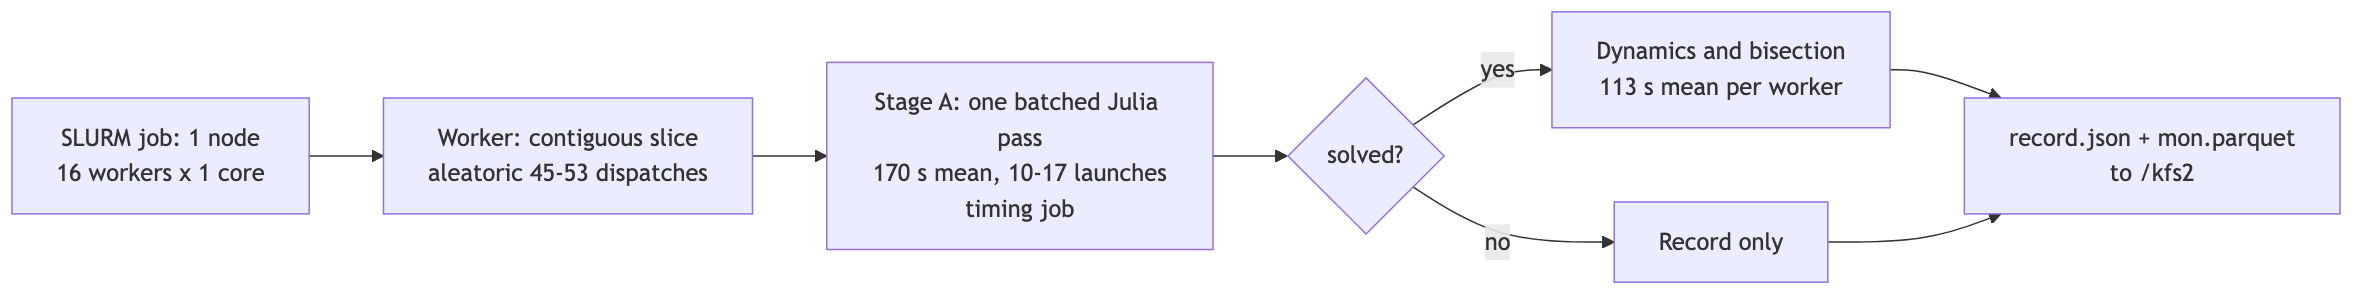
\includegraphics[width=0.72\textwidth]{figs/fig:6_per_worker_aleatoric_means_fault_sweep.png}
  \par\vspace{0.4em}
  {\small Figure 6.1. Per worker, aleatoric means. Fault sweep: stage A 122 s, dynamics 92 s.}
\end{figure}


Launch counts from the timing job, not the campaign logs.*


\subsection{Results}
\label{sec:results}

\begin{quote}
\textbf{Details for this section:}
main results, both campaigns $\cdot$
\texttt{aleatoric1\_\allowbreak{}ap08\_\allowbreak{}qlim} run $\cdot$
earlier campaign results, moved from this report $\cdot$
\texttt{phase3b} pilot $\cdot$
\texttt{faultscreen1} (alphaP 0.2, unlimited Q) $\cdot$
Phase 1 go/no-go gate $\cdot$
\texttt{inertia\_\allowbreak{}MWs} undercount bug and its correction
\end{quote}

\subsubsection{Sampling space and the two main campaigns}

Both main campaigns use the operating-condition design of {\textsection}4.2, where an operating condition is an (hour, commitment) pair. Both use DC OPF dispatch, then AC power flow with PV$\to$PQ switching ({\textsection}4.2), the datacenter as an 80/20/0 ZIP device added on top of the host load ({\textsection}4.4), and alphaP 0.8. They differ in what else varies:


\vspace{0.25cm}
\centering\small
\renewcommand{\arraystretch}{1.25}
\begin{tabularx}{\textwidth}{l >{\raggedright\arraybackslash}X >{\raggedright\arraybackslash}X}
\toprule
     & \textbf{Aleatoric campaign} \texttt{aleatoric1\_\allowbreak{}ap08\_\allowbreak{}qlim} & \textbf{Fault campaign} \texttt{faultscreen1\_\allowbreak{}ap08\_\allowbreak{}qlim} \\
\midrule
    purpose & how much operating conditions move CCT & which fault locations and placements matter \\
    hours & 20 (4 per net-load quintile) & 10 (2 per net-load quintile) \\
    operating conditions (hour, commitment) & 40 & 20 \\
    fault locations & 1 (bus 66) & 17 \\
    placements & none, or bus 6, 120, 108, 148 & none, or bus 108, 148 \\
    datacenter size & 50, 100, 200, 300, 400 MW & 200 MW \\
    runs & 840 = 40 baseline + 800 datacenter & 1,020 = 340 baseline + 680 datacenter \\
    solved & 439 (40 baseline, 399 datacenter) & 767 (340 baseline, 427 datacenter) \\
    no outcome & 401 (45 \texttt{sim\_\allowbreak{}failed}, 356 at dispatch) & 253 (168 \texttt{sim\_\allowbreak{}failed}, 85 at dispatch) \\
    datacenter runs censored at the 0.5 s cap & 121 of 399 (30.3\%) & 306 of 427 (71.7\%) \\
\bottomrule
\end{tabularx}
\vspace{0.25cm}
\normalsize\raggedright


The aleatoric campaign varies operating conditions, placement and size, at one fault. The fault campaign varies fault location and placement, at one size. \textbf{No outcome} means the run did not dispatch or did not simulate. It is reported as such, never as stable or unstable.

\subsubsection{Reading the curves: Kaplan--Meier and censoring}

Each curve estimates \textbf{$P(\mathrm{CCT} < t)$}: the share of operating conditions in which a fault cleared at $t$ seconds would be unstable. A run still stable at the 0.5 s simulation cap is \textit{censored}: we know $\mathrm{CCT} \ge 0.5$ s, not its value. The Kaplan--Meier (KM) estimator \cite{KaplanMeier1958} uses censored runs correctly:


\[
\hat S(t)=\prod_{t_i\le t}\Bigl(1-\frac{d_i}{n_i}\Bigr),\qquad \widehat P(\mathrm{CCT}<t)=1-\hat S(t)
\]

Here the $t_i$ are the distinct measured CCT values, $d_i$ is the number of runs measured at $t_i$, and $n_i$ is the number still at risk at $t_i$ (runs measured at or after $t_i$, plus censored runs). No measured CCT exceeds the cap, so for $t < 0.5$ s the estimate is simply the number of runs measured below $t$, divided by all solved runs, with the censored runs left in the denominator. No-outcome runs are excluded, so every curve is conditional on the run having solved. Figures plot the complement, $P(\mathrm{CCT} > t)$.

\begin{quote}
\textbf{Worked example:} ten made-up CCTs, with two censored runs, and the calculation step by step (illustrative values, not campaign data).
\end{quote}

The rest of {\textsection}7 runs as follows. {\textsection}7.2 works one matched example, and {\textsection}7.2b puts the 37- and 171-condition curves side by side. {\textsection}7.3 asks what adding operating conditions does to the estimate, using both pools. {\textsection}7.4 splits risk by net load. {\textsection}7.5 reports the fault sweep. {\textsection}7.6 quantifies censoring. {\textsection}7.7 covers the earlier campaigns and alphaP.

\subsubsection{A simple example: one bus, one size, one fault}

\textbf{Sampling:} \texttt{aleatoric1\_\allowbreak{}ap08\_\allowbreak{}qlim}, 200 MW at bus 108, fault at bus 66. Of the 40 operating conditions, 37 solve with the datacenter. The baseline is the same 37 conditions with no datacenter.

\textbf{Greenwood interval.} Greenwood's formula \cite{Greenwood1926} estimates the variance of a KM estimate: $\widehat{\mathrm{Var}}\big(\hat S(t)\big)=\hat S(t)^2\sum_{t_i\le t}\frac{d_i}{n_i(n_i-d_i)}$, with $d_i$ and $n_i$ as in {\textsection}7.1. We report $\mathrm{SE}=\sqrt{\widehat{\mathrm{Var}}}$. The 95\% interval is $\hat P\pm 1.96\,\mathrm{SE}$, with $\hat P=1-\hat S(t)$ (the plain interval, not log--log).


\vspace{0.25cm}
\centering\small
\renewcommand{\arraystretch}{1.25}
\begin{tabularx}{\textwidth}{l >{\raggedright\arraybackslash}X >{\raggedright\arraybackslash}X}
\toprule
     & no datacenter & 200 MW at bus 108 \\
\midrule
    operating conditions (matched) & 37 & 37 \\
    censored at 0.5 s & 46\% & 22\% \\
    \textbf{P(CCT \textless{} 0.25 s)} & \textbf{0.49} & \textbf{0.73} \\
    95\% Greenwood CI for P(CCT \textless{} 0.25 s) & 0.325--0.648 & 0.587--0.873 \\
    KM median CCT & 0.27 s & 0.18 s \\
\bottomrule
\end{tabularx}
\vspace{0.25cm}
\normalsize\raggedright


\begin{figure}[htb]
  \centering
  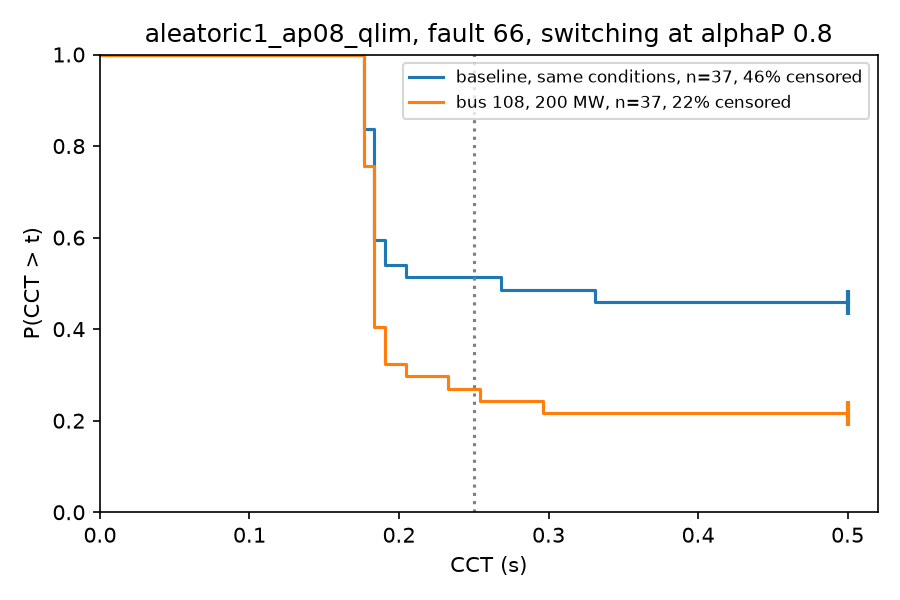
\includegraphics[width=0.85\textwidth]{figs/main_aleatoric_km_simple.png}
  \par\vspace{0.4em}
  {\small Figure 7.2. Kaplan--Meier P(CCT \textgreater{} t) on the same 37 operating conditions, without the datacenter (blue) and with the 200 MW datacenter at bus 108 (orange), fault at bus 66. Curves run to the 0.5 s cap. A censored run is still stable at the cap, so its curve holds at that value, and the tick at 0.5 s marks the censored share.}
\end{figure}


On these conditions the datacenter shortens CCT: P(CCT \textless{} 0.25 s) rises from 0.49 to 0.73. Three of the 40 conditions did not solve with the datacenter, and their baseline CCT is censored. Counting all three as CCT $\ge$ 0.25 s gives 27 of 40 (0.675). Counting all three as below 0.25 s gives 30 of 40 (0.75). The direction holds, but on this sample the size of the shift is uncertain by about 0.07.

\begin{quote}
\textbf{Working hypothesis for the direction.} The datacenter adds 200 MW to bus 108, on top of the unchanged constant-impedance host load, and 80\% of that added load does not fall with voltage. During the fault the added load keeps drawing its power, where a constant-impedance load of the same size would fall, which pushes the generators harder. The alphaP sensitivity ({\textsection}7.7) does not separate the two. It varied the P/I split with Z at zero, and CCT barely moved. So the presence of non-impedance load, rather than the P/I split within it, is the likely driver. This is not tested here. A run with the same 200 MW at a fixed impedance share would test it.
\end{quote}

\subsubsection{The same example at 37 and 171 operating conditions}

\textbf{Sampling:} bus 108, 200 MW, fault at bus 66, against the matched baseline on the same conditions. Left: \texttt{aleatoric1\_\allowbreak{}ap08\_\allowbreak{}qlim}, 37 conditions (the {\textsection}7.2 sample). Right: \texttt{aleatoric2\_\allowbreak{}ap08\_\allowbreak{}qlim}, 171 conditions (60 hours $\times$ 3 commitments, of which 171 solve with the datacenter). The two campaigns share no conditions, so they are independent samples.


\vspace{0.25cm}
\centering\small
\renewcommand{\arraystretch}{1.25}
\begin{tabularx}{\textwidth}{l >{\raggedright\arraybackslash}X >{\raggedright\arraybackslash}X}
\toprule
     & 37 conditions ({\textsection}7.2) & 171 conditions \\
\midrule
    no datacenter: P(CCT \textless{} 0.25 s), 95\% Greenwood CI & 0.486 (0.325--0.648) & 0.515 (0.440--0.590) \\
    200 MW at bus 108: P(CCT \textless{} 0.25 s), 95\% Greenwood CI & 0.730 (0.587--0.873) & 0.731 (0.665--0.797) \\
    censored at 0.5 s, no datacenter / bus 108 & 46\% / 22\% & 42\% / 14\% \\
\bottomrule
\end{tabularx}
\vspace{0.25cm}
\normalsize\raggedright


\begin{figure}[htb]
  \centering
  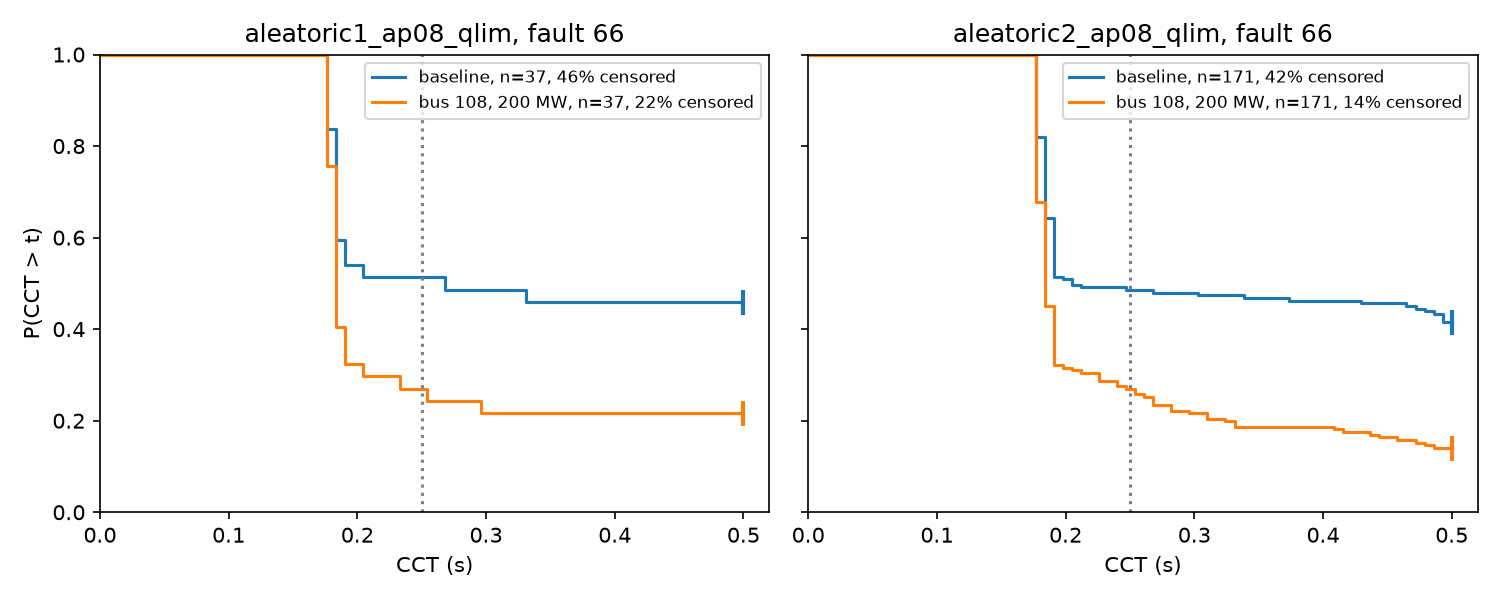
\includegraphics[width=0.85\textwidth]{figs/main_km_37_vs_171.png}
  \par\vspace{0.4em}
  {\small Figure 7.2b. Kaplan--Meier P(CCT \textgreater{} t) at bus 108, 200 MW (orange) against the matched baseline (blue), fault at bus 66. Left: 37 conditions (\texttt{aleatoric1}). Right: 171 conditions (\texttt{aleatoric2}). Same axes in both panels, curves run to the 0.5 s cap, and the tick at 0.5 s marks the censored share. With 171 conditions the curve has about 4.6 times as many conditions behind each step, so it resolves finer structure and the interval at 0.25 s is narrower.}
\end{figure}


Two points. First, the datacenter moves P(CCT \textless{} 0.25 s) from about 0.5 to 0.73 in both campaigns (the two panels). Second, the datacenter-arm interval is 0.132 wide at 171 conditions, against 0.287 at 37, the narrowing expected from the larger sample. The interval describes the procedure: if the study were repeated with new samples of conditions, about 95\% of intervals built this way would contain the true P. It does not give a 95\% probability that the true value lies in this one. Overlap of two separate intervals is not a test of a difference. The arms are matched on the same conditions, so a difference needs a paired interval, which we have not computed. Nine of the 180 conditions did not solve with the datacenter (8 solve failures, 1 simulation failure) and are excluded from the 171. {\textsection}7.3 gives a related check on how the estimate settles as conditions are added.

\subsubsection{More operating conditions: how the estimate settles}

We checked whether the estimate stops moving as conditions are added, by recomputing it on random subsets of each pool (\textit{subsampling} \cite{PolitisRomano1994}; references and details in the plan). For bus 108, 200 MW, the median over 2,000 random orderings settles at 0.730--0.733 from about 30--37 conditions in both pools. This holds for these two pools only, and the check does not give an uncertainty; that is the Greenwood interval in {\textsection}7.2b. The campaign did not need it, because all samples are already used. We might use the same check later as an alternative way to size a future study, if a full-size design costs too much. The plan sets out how.


\begin{figure}[htb]
  \centering
  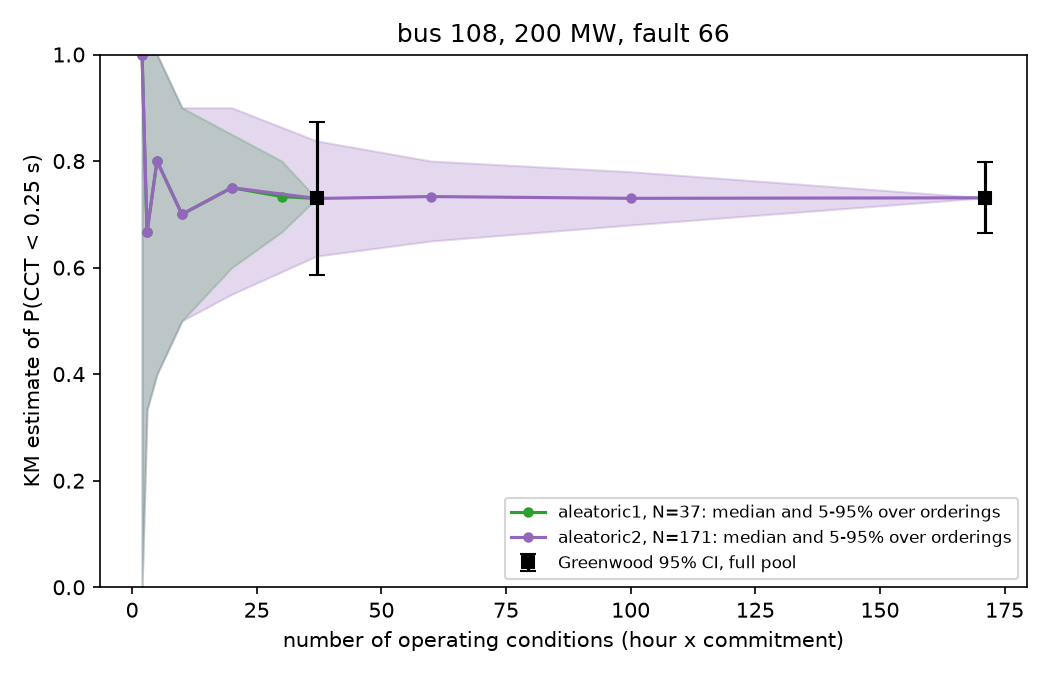
\includegraphics[width=0.85\textwidth]{figs/main_convergence_37_vs_171.png}
  \par\vspace{0.4em}
  {\small Figure 7.3. KM estimate of P(CCT \textless{} 0.25 s) at bus 108, 200 MW, over random orderings of the 37-condition pool (green) and the 171-condition pool (purple). Line: median over 2,000 orderings. Shading: 5th--95th percentile. Black squares: full-pool estimate with its 95\% Greenwood interval. Both medians sit at 0.730--0.733 from about 30--37 conditions onward. This is a check on these two pools only.}
\end{figure}


The spread of CCT across conditions does not shrink with more samples. Adding conditions shrinks the error in the probability; the spread is a property of the conditions, and reducing it needs conditioning on something that explains it, such as net load ({\textsection}7.4). Within the two highest net-load quintiles every measured CCT lies between 0.177 and 0.191 s, while the lower quintiles range up to 0.49 s.

\subsubsection{Risk by net load}

\textbf{Sampling:} \texttt{aleatoric1\_\allowbreak{}ap08\_\allowbreak{}qlim}, datacenter at buses 6, 120, 108 and 148, at 50 to 400 MW, one fault. Hours are split into five net-load quintiles of 4 hours each. Each quintile holds 160 datacenter runs (4 buses $\times$ 5 sizes $\times$ 4 hours $\times$ 2 commitments).


\vspace{0.25cm}
\centering\small
\renewcommand{\arraystretch}{1.25}
\begin{tabularx}{\textwidth}{l >{\raggedright\arraybackslash}X >{\raggedright\arraybackslash}X >{\raggedright\arraybackslash}X >{\raggedright\arraybackslash}X >{\raggedright\arraybackslash}X}
\toprule
    quintile & mean net load (MW) & datacenter runs solved & no outcome & censored & \textbf{P(CCT \textless{} 0.25 s)} \\
\midrule
    q0 & 1,009 & 75 of 160 & 85 & 83\% & \textbf{0.07} \\
    q1 & 1,201 & 82 of 160 & 78 & 72\% & \textbf{0.16} \\
    q2 & 1,421 & 82 of 160 & 78 & 0\% & \textbf{0.73} \\
    q3 & 1,677 & 80 of 160 & 80 & 0\% & \textbf{1.00} \\
    q4 & 1,860 & 80 of 160 & 80 & 0\% & \textbf{1.00} \\
\bottomrule
\end{tabularx}
\vspace{0.25cm}
\normalsize\raggedright


\begin{figure}[htb]
  \centering
  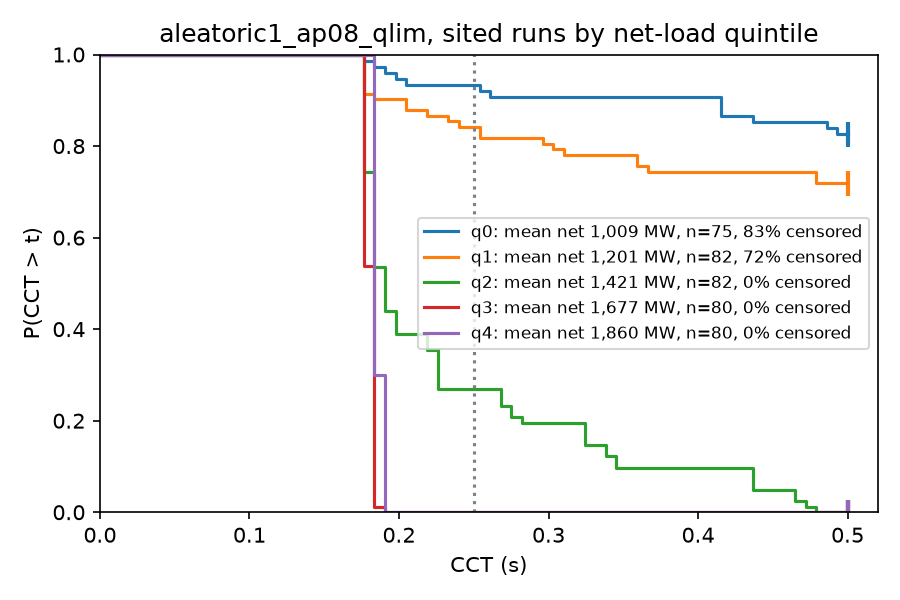
\includegraphics[width=0.85\textwidth]{figs/main_aleatoric_km_by_netload.png}
  \par\vspace{0.4em}
  {\small Figure 7.4. Kaplan--Meier P(CCT \textgreater{} t) by net-load quintile, datacenter runs only (all buses and sizes), fault 66.}
\end{figure}


P(CCT \textless{} 0.25 s) climbs from 0.07 in the lowest quintile to 1.00 in the two highest, with the step between q1 (mean 1,201 MW) and q2 (mean 1,421 MW). Conditioning on net load therefore accounts for the spread in {\textsection}7.3.

\begin{itemize}
  \item \textbf{Conditional on solving.} Between 49\% and 53\% of datacenter runs in each quintile have no outcome. Whether the no-outcome runs would have the same CCT is unknown.
  \item \textbf{Dispatch failures are spread across quintiles} (68 to 77 each), unlike the fault campaign ({\textsection}7.5).
  \item \textbf{Baseline has only 8 solved runs per quintile}, too few for a quintile estimate. The matched comparison is in {\textsection}7.2.
\end{itemize}

\subsubsection{The fault sweep: what it measures and which faults discriminate}

\textbf{Sampling:} \texttt{faultscreen1\_\allowbreak{}ap08\_\allowbreak{}qlim}, the fault sweep. 10 hours (2 per net-load quintile) $\times$ 2 commitments $\times$ 17 fault locations. There are 340 baseline runs with no datacenter, all solved, and 680 runs with a 200 MW datacenter at bus 108 or 148.


\vspace{0.25cm}
\centering\small
\renewcommand{\arraystretch}{1.25}
\begin{tabularx}{\textwidth}{l >{\raggedright\arraybackslash}X >{\raggedright\arraybackslash}X}
\toprule
     & baseline (no datacenter) & datacenter (200 MW) \\
\midrule
    solved & 340 of 340 & 427 of 680 \\
    censored at 0.5 s & 302 (88.8\%) & 306 (71.7\%) \\
    no outcome & --- & 253: 168 \texttt{sim\_\allowbreak{}failed} (97 at alphaP 0.8 only, 71 at both alphaP levels), 85 at dispatch \\
\bottomrule
\end{tabularx}
\vspace{0.25cm}
\normalsize\raggedright


Matched by (hour, commitment, fault), using datacenter runs that solved:

\begin{itemize}
  \item \textbf{Bus 108}, 194 pairs: P(CCT \textless{} 0.25 s) is 0.072 with the datacenter and 0.041 without. Censored: 70\% and 81\%.
  \item \textbf{Bus 148}, 233 pairs: 0.064 and 0.034. Censored: 73\% and 84\%.
  \item The datacenter is measured where the baseline is censored in 22 pairs (bus 108) and 25 pairs (bus 148). The reverse happens in none.
  \item Where both runs are measured, the pairs cover the same 37 conditions at both buses, because the baseline is measured on only 38 conditions. The median $\Delta$CCT is 0 s, 5 of 37 pairs fall with the datacenter, and the largest drop is 0.24 s.
\end{itemize}

Reading: on this campaign the datacenter raises P(CCT \textless{} 0.25 s) only slightly, from 0.04 to 0.07 at bus 108 and from 0.03 to 0.06 at bus 148. Most baseline runs are censored (81--84\% on these pairs), so the signal is weak. The direction matches {\textsection}7.2, which uses a different fault and a measured baseline.

\begin{quote}
\textbf{Working hypothesis for the 97 runs that fail only at alphaP 0.8.} These are datacenter runs that solve at alphaP 0.2 and fail at alphaP 0.8: 89 at initialization and 8 in the transient. The constant-power share may move the fault-on dispatch past a bolted fault, so no post-fault start exists. This is supported on one dispatch (h1879), not established elsewhere, and can be falsified. The predictions, and the breakdown of the 71 shared failures and the 85 dispatch failures, are in the issue doc {\textsection}9 and the plan. Report these runs as no outcome.
\end{quote}

All 85 dispatch failures fall in q0, the lowest net-load quintile: 85 of its 136 datacenter runs, or 63\%. No dispatch failure occurs in q1 to q4. The cause of the q0 concentration has not been checked.

Baseline CCT by fault location, for the 20 baseline conditions each:


\vspace{0.25cm}
\centering\small
\renewcommand{\arraystretch}{1.25}
\begin{tabularx}{\textwidth}{l >{\raggedright\arraybackslash}X >{\raggedright\arraybackslash}X >{\raggedright\arraybackslash}X}
\toprule
    fault bus & median baseline CCT & censored & measured of 20 \\
\midrule
    \textbf{94} & \textbf{0.37 s} & \textbf{35\%} & \textbf{13} \\
    66 & 0.5 s (cap) & 55\% & 9 \\
    68 & 0.5 s (cap) & 60\% & 8 \\
    181 & 0.5 s (cap) & 60\% & 8 \\
    other 13 & 0.5 s (cap) & 100\% & 0 \\
\bottomrule
\end{tabularx}
\vspace{0.25cm}
\normalsize\raggedright


\begin{figure}[htb]
  \centering
  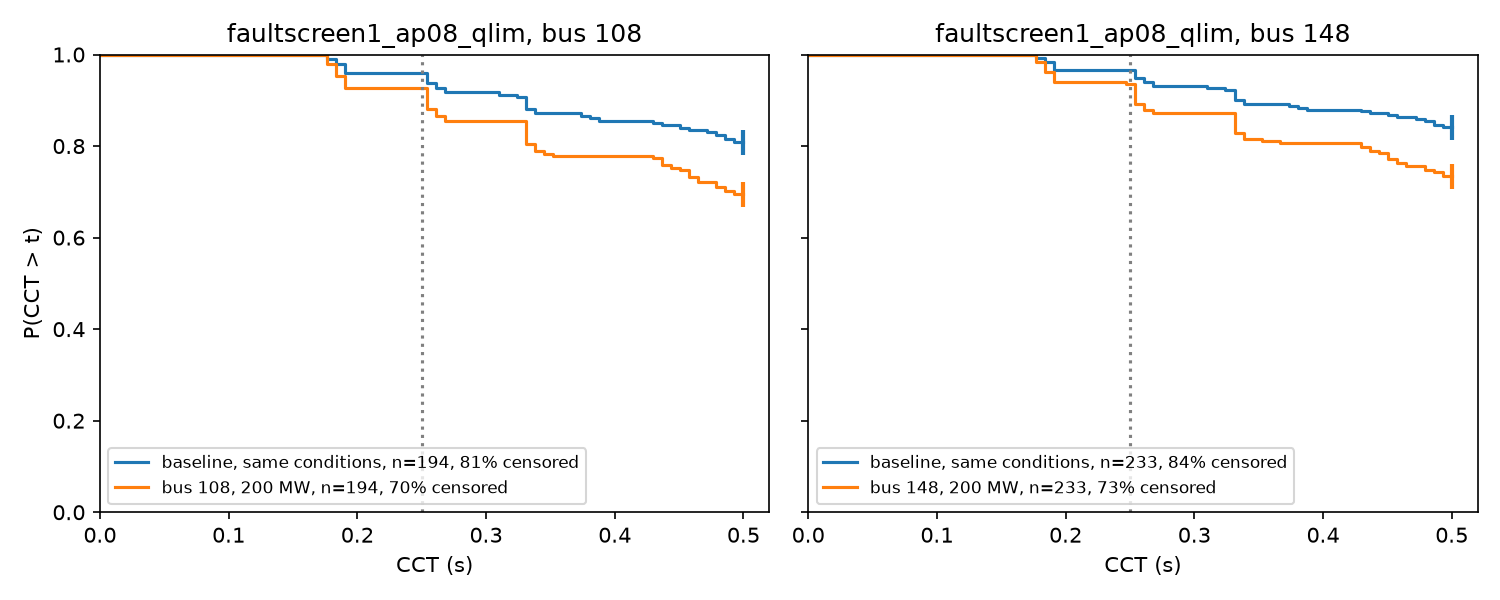
\includegraphics[width=0.85\textwidth]{figs/main_faultscreen_km.png}
  \par\vspace{0.4em}
  {\small Figure 7.5. Kaplan--Meier P(CCT \textgreater{} t) for the datacenter at bus 108 (left) and bus 148 (right), each against the baseline on the same matched (hour, commitment, fault) conditions. Baseline in blue, datacenter in orange.}
\end{figure}


Thirteen of 17 fault locations are censored in every baseline condition, so a uniform fault budget spends most of its runs on faults that cannot separate operating conditions. Fault screening should be cheap, followed by concentration on the informative faults; the plan has the design detail. Bus 66, the fault in the aleatoric campaign, is not the most informative location: bus 94 is. At 200 MW, buses 108 and 148 look alike in this sample (0.072 against 0.064 for P(CCT \textless{} 0.25 s)).

\subsubsection{Censoring: dropping censored runs inflates risk}

Dropping censored runs from a risk estimate inflates it by a factor that depends only on the censored share, not on the threshold:


\vspace{0.25cm}
\centering\small
\renewcommand{\arraystretch}{1.25}
\begin{tabularx}{\textwidth}{l >{\raggedright\arraybackslash}X >{\raggedright\arraybackslash}X >{\raggedright\arraybackslash}X >{\raggedright\arraybackslash}X}
\toprule
    campaign & datacenter runs solved & measured & censored share & inflation from dropping censored runs \\
\midrule
    \texttt{aleatoric1\_\allowbreak{}ap08\_\allowbreak{}qlim} & 399 & 278 & 30.3\% & \textbf{1.44$\times$} \\
    \texttt{faultscreen1\_\allowbreak{}ap08\_\allowbreak{}qlim} & 427 & 121 & 71.7\% & \textbf{3.53$\times$} \\
\bottomrule
\end{tabularx}
\vspace{0.25cm}
\normalsize\raggedright


\[
\frac{\hat P_{\text{drop}}}{\hat P_{\text{keep}}} = \frac{N_{\text{solved}}}{N_{\text{measured}}}
\]

This follows from {\textsection}7.1, since censoring sits at one point beyond every measured value. The factor is arithmetic, but it is easy to get wrong by quoting one population's censored share against another's label. The 3.53$\times$ corresponds to 71.7\% censoring among datacenter runs that solved. It is not the share of the 1,020 planned runs.

\par\vspace{0.4em}
\noindent\fbox{\parbox[t]{0.98\textwidth}{%
\setlength{\parskip}{0pt}%
\textbf{Details:} \url{https://github.com/ORNL/GridKit/blob/isatkaus/uq-usecase/uq-usecase/work-notes/datacenter_load_uq_plan.md}. Sections: "alphaP tested as a sensitivity", "the feasible-alphaP frontier, mapped", "fault location is the missing variable", "phase3b siting pilot and earlier campaigns"
}}
\vspace{0.2em}


\subsection{First look at ACTIVSg2000}
\label{sec:first_look_activsg2000}

The 200-bus case is small enough that brute force works: whole campaigns finish in minutes. That is convenient but it hides the question the methods work exists to answer, so before pausing we measured what changes at \textbf{ACTIVSg2000} (2,000 buses, the TAMU synthetic Texas case \cite{TAMUrepo}). This is scoping, not a campaign.

\textbf{What already exists.} A GridKit \texttt{case.json} ships with the repo, raw TAMU data and processed hourly \texttt{demand} / \texttt{wind} / \textbf{\texttt{solar}} profiles are on \texttt{/projects}. The base case \textbf{runs unmodified}: a 10 s simulation with a 0.15 s fault completes with \texttt{rc = 0} at both default and full monitoring.

\textbf{Measured, same settings on both cases.} Stage-A figures are warm per-case \texttt{solve\_\allowbreak{}time} from one batched Julia process, so the ~6 s launch is amortised rather than counted; cold single-shot timings are launch-dominated and misleading.


\vspace{0.25cm}
\centering\small
\renewcommand{\arraystretch}{1.25}
\begin{tabularx}{\textwidth}{l >{\raggedright\arraybackslash}X >{\raggedright\arraybackslash}X >{\raggedright\arraybackslash}X}
\toprule
    quantity & ACTIVSg200 & ACTIVSg2000 & ratio \\
\midrule
    buses & 200 & 2,000 & 10$\times$ \\
    branches & 246 & 3,206 & 13$\times$ \\
    devices & 476 & 5,787 & 12.2$\times$ \\
    synchronous machines & 40 & 334 & 8.4$\times$ \\
    \texttt{LoadZIP} & 109 & 1,245 & 11.4$\times$ \\
    \texttt{case.json} & 0.24 MB & 2.93 MB & 12.2$\times$ \\
    \textbf{DC OPF} (warm) & 0.011 s & 0.212 s & \textbf{19.1$\times$} \\
    \textbf{AC PF} (warm) & 0.018 s & 0.331 s & \textbf{18.5$\times$} \\
    \textbf{stage A total} & 0.029 s & 0.543 s & \textbf{18.7$\times$} \\
    \textbf{one dynamic run} (solver time), full monitors & 0.28 s & 7.08 s & \textbf{25.3$\times$} \\
    monitor CSV & 27.3 MB & 262.5 MB & 9.6$\times$ \\
    monitor columns & 481 & 4,649 & 9.7$\times$ \\
\bottomrule
\end{tabularx}
\vspace{0.25cm}
\normalsize\raggedright


\textbf{The shape of the growth.} Against a 10$\times$ increase in buses, data scales \textbf{linearly} ($\approx N^{1.0}$), stage A as $\approx N^{1.27}$, and the dynamic simulation as $\approx N^{1.40}$. So compute grows faster than the network and faster than storage, and the dynamic stage --- the cheap one at 200 buses --- grows fastest.

\textbf{What that implies for a campaign.} Projecting \texttt{aleatoric1} (840 conditions, one full run plus ~8 bisection probes each, so ~7,560 simulations). Serial times use the measured per-run cost; wall times assume the pilot's 16 workers per node and scale linearly, which is optimistic until per-worker memory is known:


\vspace{0.25cm}
\centering\small
\renewcommand{\arraystretch}{1.25}
\begin{tabularx}{\textwidth}{l >{\raggedright\arraybackslash}X >{\raggedright\arraybackslash}X}
\toprule
     & ACTIVSg200 & ACTIVSg2000 \\
\midrule
    per dynamic run (solver time), full monitors, \texttt{tmax} 10 s & 0.28 s & \textbf{7.08 s} \\
    stage A, all 840 conditions & 24 s & 456 s \\
    \textbf{dynamic runs, serial} & \textbf{~35 min} & \textbf{~14.9 h} \\
    wall on 1 node, 16 workers & ~2.2 min & \textbf{~56 min} \\
    wall on 1 node, 32 workers & ~1.1 min & \textbf{~28 min} \\
    monitor output, raw CSV & 22 GB & \textbf{~220 GB} \\
    after parquet & 4.5 GB & \textbf{~45 GB} \\
\bottomrule
\end{tabularx}
\vspace{0.25cm}
\normalsize\raggedright


\textit{(Calibration: \texttt{aleatoric1} took 6.0 min of wall on one node with 16 workers (SLURM job 19813984). The ideal for the same job is 2.2 min, so the measured overhead is about 2.7$\times$, from scheduling, startup and per-launch cost. Applied to the 2000-bus ideal, a full-size campaign is about \textbf{2.5 h of wall on one node at 16 workers}, not under one node-hour. These are projections, not measurements.)}

Compute is still affordable, but it is not negligible. At 200 buses the 104 cores bind before memory does: at 0.88 GB per worker, 246 GB would allow about 280 workers before OS overhead. The 16 workers per node were the pilot's choice, not a hard limit. At 2000 buses one dynamic run peaked at 126 MB and a two-case stage-A batch at 1.0 GB, but a full worker batch is \textbf{unmeasured}, so it is the number to measure before relying on any wall-time projection. Until then, treat ~2.5 h (calibrated, one node, 16 workers) as the planning number. \textbf{Storage, not compute, is the binding constraint}, and the mitigation is already known: 4,000 of the 4,649 columns are bus \texttt{Vr}/\texttt{Vi}, so selective monitoring is worth far more here than it was at 200 buses, where the same trick already bought 13.8$\times$ on bisection probes.

\textbf{Why this matters for the methods work.} The \textit{design space} grows along two axes: siting candidates about 11.5$\times$ (108 load buses to 1,245) and fault locations 10$\times$ (200 to 2,000), roughly 115$\times$ more design points, while per-sample cost grows 19--25$\times$. Holding sampling \textit{density} fixed projects to roughly \textbf{2,150--2,900$\times$} the pilot's cost (a projection, not a measurement). Brute force survives one order of magnitude, not two. The execution model also inverts: at 200 buses it exists to amortise an expensive dispatch over cheap disturbances, whereas at 2,000 buses the dynamic run dominates and the quantity to minimise becomes the \textit{number of simulations}, not the number of dispatches. That is the concrete case for screening, surrogates and adaptive refinement over a larger factorial, and it makes the pilot's measured 76 \% contingency waste far more expensive to tolerate.

Porting the pipeline to 2,000 buses surfaced one blocker --- in our campaign code, not GridKit's, now fixed and verified end to end. The case mixes machine, exciter and governor classes the 200-bus pipeline never saw; 101 online units carry no dynamic model and are handled as the same negative-load stand-in used for wind; and positional unit ids at the 13 multi-generator buses hid a dispatch-mapping bug (\texttt{match\_\allowbreak{}gens\_\allowbreak{}by\_\allowbreak{}mva} on \texttt{(bus, MBASE)} fixes it) that a 200-bus case is too small to expose. A \texttt{faultscreen}-shaped micro-campaign already runs on the case.

The pilot's aleatoric campaign is a 40-condition grid. A campaign at this scale needs distributions over more wind and load conditions, more placements and more fault buses, with spatial structure, which brute force will not reach. The pilot already shows where the leverage is: the estimate of P(CCT \textless{} 0.25 s) has a standard error of about 0.07 at 37 conditions ({\textsection}7.2), and CCT spread is concentrated by net-load quintile ({\textsection}7.4), so conditioning and stratification --- not simply more samples --- are what tighten the answer. \texttt{aleatoric2} (SLURM 19830145: 3,780 design rows, 1,958 solved, 17.1 min on one node, 9.9 GB stored) already measured how cost scales with the sample count. The question becomes \textit{which} dynamic runs to spend, which is where {\textsection}9 takes up.

\par\vspace{0.4em}
\noindent\fbox{\parbox[t]{0.98\textwidth}{%
\setlength{\parskip}{0pt}%
\textbf{Details:} \url{https://github.com/ORNL/GridKit/blob/isatkaus/uq-usecase/uq-usecase/work-notes/datacenter_load_uq_plan.md}. Sections: "scaling measurements, the ACTIVSg2000 port, and the positional-id trap", "sampling at scale and the sampling dimensions", "working with ACTIVSg2000"
}}
\vspace{0.2em}


\subsection{Where this goes}
\label{sec:where_this_goes}

The pilot leaves a clear picture of where cost lives and therefore where the methods work should go. At 200 buses the expensive part is \textbf{stage A}, and the scientifically interesting dimensions --- contingency location, disturbance severity, model form --- are nearly free once a dispatch exists. At 2,000 buses ({\textsection}8) that asymmetry inverts: the dynamic run dominates, the design space grows by two orders of magnitude, and the quantity to minimise becomes the number of simulations. Making aleatoric UQ affordable at that scale is \textbf{FY27 planned work}, pursued along two complementary tracks.

\textbf{Track 1 --- spend fewer, better-chosen dynamic runs.} The pilot already measured the levers:

\begin{enumerate}
  \item \textbf{Screen contingencies cheaply, then concentrate.} 76 \% of a uniform fault budget was wasted here ({\textsection}7.5), with 13 of 17 locations fully censored. On a 10k-bus case the contingency list is the part that explodes and also the part that is free to explore.
  \item \textbf{Treat censoring as information.} Both "survived beyond the cap" and "infeasible" are results, and at high censoring they are most of the dataset. A cheap 1--2 run classifier that detects the censored case before committing to an 8-run CCT bisection would remove most of the cost.
  \item \textbf{Condition and stratify, rather than only adding samples.} CCT spread is largely explained by net load ({\textsection}7.4), so stratified or importance sampling on net load cuts variance at fixed cost; a variance decomposition of the existing 840 runs is a zero-cost first step.
  \item \textbf{Surrogate or warm-started CCT, and early-terminating integration.} Neighbouring dispatches have strongly correlated CCT, and pole slip is detectable well before \texttt{tmax}, so both the number and the length of simulations can be cut.
  \item \textbf{Exploit the conditional-independence structure.} Expensive outer samples over operating conditions, cheap inner fan-out over disturbances and model parameters --- the same motivation as multilevel Monte Carlo \cite{Giles2015}, driven by model structure rather than discretisation.
\end{enumerate}

\textbf{Track 2 --- a graph surrogate, as an alternative and supplement to sampling.} The grid is intrinsically a graph: the admittance matrix is a weighted Laplacian over buses, a fault propagates through branch impedances as a message-passing process, and "which bus to site load at" is itself a graph question. Graph neural networks and graph transformers carry exactly that inductive bias \cite{Battaglia2018}, and have been used as fast power-system surrogates \cite{Donon2020}. A surrogate trained on the records the sampling campaigns already produce --- the \texttt{(graph, operating point, parameters, fault)} $\to$ trajectory map --- could emulate CCT or the stability label cheaply, turning the expensive solver into a screening oracle and reserving dynamic runs for confirmation and for labelling the cases where the surrogate is least certain, an active-learning loop \cite{Settles2009} that chooses which runs to spend. This is \textbf{supplemental} to sampling-based UQ, not a replacement: the surrogate lowers per-sample cost, while the sampling design still fixes what the estimate means. Our fuller survey of these ideas is in \texttt{gt\_\allowbreak{}ideas.md}.

The near-term steps are the cheap ones: a wider contingency screen, a paired-censoring treatment of \texttt{dCCT}, a variance decomposition of the existing runs, a short literature check on datacenter load modelling so {\textsection}10's constraint can be addressed rather than worked around, and porting \texttt{CampaignConfig} to ACTIVSg2000 ({\textsection}8). The graph-surrogate track builds on the dataset those campaigns are already generating.

\par\vspace{0.4em}
\noindent\fbox{\parbox[t]{0.98\textwidth}{%
\setlength{\parskip}{0pt}%
\textbf{Details:} \url{https://github.com/ORNL/GridKit/blob/isatkaus/uq-usecase/uq-usecase/work-notes/datacenter_load_uq_plan.md}. Sections: "where numerical-methods contributions could be made"
}}
\vspace{0.2em}


